\chapter{基于并行的知识图谱与文本模型联合学习框架}
\label{cha3:jointlearning}

\section{章节引言}

我们之前介绍过,典型的知识图谱是一个多关系有向图,其节点对应于现实世界中的抽象实体,边对应于抽象实体间的复杂关联。知识图谱中的事实通常以关系三元组的形式存在,如$(h, r, t)$,$h$和$t$表示\emph{头}实体和\emph{尾}实体,$r$表示$h$和$t$之间的\emph{关系}。例如(\emph{马克·吐温},\emph{出生于},\emph{佛罗里达州})。

不过目前的知识图谱还远远达不到完善的程度,尽管它们规模已经很庞大了。通常有两类任务来获取知识信息并以此拓展知识图谱,知识图谱填充以及关系抽取。知识图谱填充旨在通过图谱内部的网络空间结构来挖掘信息并推测新的事实三元组,其中包括了基于图结构的模型\cite{lao2010relational,lao2011random},基于张量的模型\cite{socher2013reasoning, nickel2016holographic},以及基于平移的模型\cite{bordes2013translating,ji2015knowledge}。与图谱填充技术不太一样,关系抽取主要是从自由文本中提取特征并用来抓取新的关系事实。在这个方向上,也有大量行之有效的工作出现。Surdeanu \cite{surdeanu2012multi}就提出了一套基于多实例和远距离监督算法的模型,成为现在大多数方法的雏形。近年来,随着深度学习的发展,Zeng \cite{zeng2014relation}使用卷积神经网络来嵌入语句特征,也获得了不错的结果。

虽然依靠的信息来源是不同的,但这两个方向的目标是一致的,即进行知识获取。因此,将知识图谱和文本语料进行融合来进行知识信息的获取是一个非常直接的想法,并且已经在过去的一些工作中被简单探索。Weston \cite{weston2013connecting}直接将两方面模型的能量函数进行加,从而最终的预测是涉及图谱和文本两方面信息的结果。Wang \cite{wang2014knowledge}提出了一个简单框架将文本的词向量和实体向量进行对齐。Toutanova \cite{toutanova2015representing} 则是从纯文本中提取文本关系并与关系向量对齐。这些模型要么只考虑了文本与图谱的部分对应关系,如单纯的实体文本对应或者关系文本对应,要么特征融合后仅仅解决了知识获取中单方面的任务,这意味着这些模型还有很多可改动的空间。另外这些方法图谱和文本的结合模式大都是串行的,神经网络巨大的运算量将会带来长时间的训练,在大规模数据上适用也值得商榷。

为了解决这些问题,我们提出了一个通用的联合框架可以同时融入知识图谱填充以及关系抽取的模型,并其联合方式是基于平行的,相比于串行联合在效率上提升很大。如图\ref{fig3:joinglearning}所示,该框架同时对单词、实体、关系以及文本关系进行了对齐,从而能够综合考虑文本和知识图谱的信息并发挥各自优势。此外,我们使用了深层神经网络与基于知识图谱的注意力机制来构建文本模型,而不是使用传统的语言分析来编码句子的语义,这非常适用于大规模文本尤其是掺杂有噪音的远距离监督抓取得到的文本。基于知识的注意力机制使用知识图谱的信息来选择语料中的最核心的句子来强化训练,与此同时,文本的关系特征也通过注意力机制反馈给图谱模型。因为只有强有力的图谱特征才能进行这样的筛选。我们的框架也是非常灵活的,大多数现有的基于嵌入式的图谱填充算法以及关系抽取算法都可以很容易地集成到框架之中。

我们在真实环境下的数据上进行了实验,其中知识图谱是从Freebase中提取获得的,而文本则是来源于纽约时代周刊的语料库。我们同时在知识图谱填充和关系抽取两个方向上进行实验评估。而实验的结果也表明,我们的框架可以有效地进行联合学习和特征融合,并获得嵌入更多信息量的知识和文本表示,其效果显著优于单一依靠图谱或者文本的基础方法。

\section{相关工作}

在本章节中,我们罗列了与框架相关的工作,包括知识图谱表示学习、文本关系表示模型、基于联合学习的知识获取模型以及基于注意力机制的神经网络模型,相关内容如下。

\subsection{知识图谱表示学习模型} 

对于知识图谱表示学习,已经有一些成熟的模型被设计出来,将图谱中的实体与关系嵌入到低维连续空间中,从而能够以数学形式刻画知识图谱的结构。Bordes \cite{bordes2013translating} 提出了基于平移的知识图谱表示学习模型 TransE,其基本假设就是将每个事实$(h, r, t)$中的关系$r$视为低维空间内的$ h$至$t$向量的平移,例如,$\textbf{h} + \textbf{r} = \textbf{t}$。尽管 TransE 的模型非常简洁,却能取得非常优异的结果,无论是效率上还是结果上。因此,大量的扩展模型也在 TransE 的基础上被提了出来,包括 TransH \cite{wang2014transh}、TransR \cite{lin2015learning}、TransD \cite{ji2015knowledge}等。除了基于平移的模型之外,基于张量的模型,诸如 RESCAL \cite{nickel2011three}、NTN \cite{socher2013reasoning}、HOLE \cite{nickel2016holographic},也是非常有效的模型。某种程度上,基于张量的模型比基于平移的模型表达能力要强一些。但是基于张量的模型训练缓慢,参数数量以及资源占用也非常大。出于时效性价比的考虑,我们将基于平移的模型 TransE 和 TransD 作为代表模型在我们的框架中进行知识图谱表示学习。

\subsection{文本关系表示学习模型}

大量的工作和模型也被提出,力图从大规模文本语料中提取关系事实。Mintz \cite{mintz2009distant} 在其工作中提出了远距离监督(Distant Supervised)模型,利用知识图谱自动标注文本数据,再利用自动标注的文本数据用以构建关系表示模型并进行关系抓取。之后,Hoffmann \cite{hoffmann2011knowledge} 在远距离监督模型的基础上提出了跨句合并机制,利用句子间的相关特征来服务抓取模型。实体间的关系往往不是唯一的,而Surdeanu \cite{surdeanu2012multi} 提出了多关系抓取模型 MIML 来解决这个问题。在最近的几年里,深度神经网络被使用在各个领域中,包括文本关系表示,其中有基于卷积神经网络的工作 \cite{zeng2014relation,zeng2015distant}、基于循环神经网络的工作 \cite{zhang2015relation}、长效记忆网络模型\cite{xu2015classifying,miwa2016end}。对于给定的句子以及句子中的实体,神经网络会将句子的语义编码为语义向量,而语义向量则可以帮助模型获取文本关系。与传统的模型相比,神经网络模型能够准确地捕获文本关系而不用进行过于复杂的语言分析和特征处理。出于时间效率上的考虑,在本工作中,我们应用卷积神经网络来嵌入文本关系。


\subsection{基于联合学习的知识获取模型}

也有一些工作尝试将知识图谱和文本语料联合在一起进行特征融合以及知识信息的获取。Weston \cite{weston2013connecting}提出了一个简单的算法。Weston将 TransE 和 文本模型进行简单结合,用文本模型的评分与知识图谱模型的评分加权和进行预测。虽然方法十分简单,但是在关系抽取上取得了巨大的成功和惊人的表现。之后,Wang \cite{wang2014knowledge} 提出了一套联合学习的框架,将词向量与知识图谱的实体向量进行关联,同步训练并在训练过程中共享参数,从而将文本特征与图谱特征进行融合。Xie \cite{xie2016representation}和 Wu \cite{wu2016knowledge} 使用神经网络将与实体相关的文本内容嵌入到图谱空间中去,从而可以强化图谱中实体的表达能力。Toutanova \cite{toutanova2015representing}使用文本依赖关系解析从纯文本中提取文本关系来增强图谱中关系嵌入的表达能力。 
在本工作中,我们结合现有的知识获取模型,建立一个统一的联合学习框架,使单词、实体和关系都进行对应,并且有别于以往串行结合的联合方式,我们采用平行的结合方式来增加训练速度。


\subsection{基于注意力机制的神经网络模型} 

注意力机制最早被Bahdanau\cite{bahdanau2014neural}在其神经机器翻译模型中使用,用来从神经网络的隐层向量里选择最重要的成分来强化训练且规避噪音。在关系抽取上,Lin\cite{lin2016neural}立足于以往的模型,通过跨句级别的注意力机制来减少远距离监督算法带入的噪音成分。在本工作中,我们提出了一种基于知识图谱的注意力机制。与Lin\cite{lin2016neural}不同,我们基于知识的注意力机制不是采用全局的注意力特征,而是使用图谱信息构建局部的注意力特征,这会在复杂的文本环境下更加有效和鲁棒。


\vspace{25pt}
\begin{figure}[h]
\setlength{\abovecaptionskip}{30pt} 
\centering
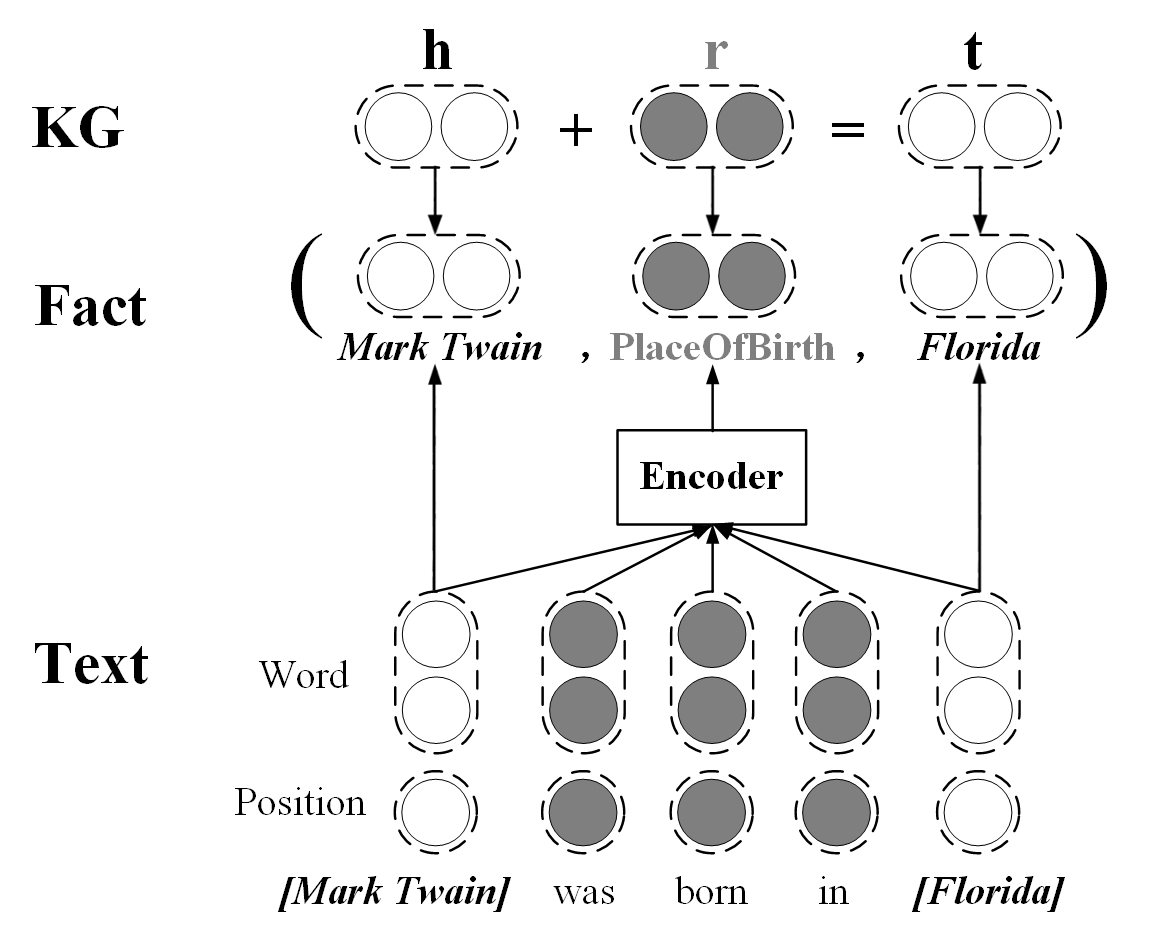
\includegraphics[width=0.8\columnwidth]{figures/ch3/joint.jpg}
\caption{基于并行的知识图谱与文本模型联合学习框架}
\label{fig3:joinglearning}
\end{figure}


\section{算法框架}
在这一章节的内容里,论文主要介绍我们提出的基于并行的知识图谱与文本模型联合学习框架。内容包括以下几点:(1)联合框架下知识图谱与文本表示的统一形式;(2)知识图谱表示学习模型;(2)文本关系表示学习模型;(3)基于知识的跨句注意力机制;(4)初始化及实现细节,整体的框架结构也可以在图\ref{fig3:joinglearning}中看到。从框架结构图中可以发现,在整个框架中,我们进行了大量的嵌入表示融合工作。这些融合工作包含了知识图谱与文本表示在模型形式上的统一,词与实体、关系与文本关系在嵌入向量上的统一等等。得益于这些统一的归纳与抽象,我们可以通过使用统一空间学习嵌入表示的方式来进行联合学习。联合学习支持模型间的参数共享,从而使得原本分离的模型在合并后可以相互影响并一定程度的促进各自效果提升。在介绍具体细节之前,我们仍然先引入一些符号体系和重要概念。

\subsection{符号体系和重要概念}

与大规模知识图谱表示学习框架一样,我们在这里同样将整个知识图谱定义为一个由实体集、关系集和事实三元组集合共同组成的大集合,即$G = \{E, R, T\}$,这里$E$、$R$和$T$分别表示实体集合、关系集合和事实三元组集合。对于事实三元组集合中的任意事实$(h, r, t) \in T$,这个三元组表明头实体$h \in E$和尾实体$t \in E$之间存在一个逻辑上的关联$r \in R$。

同知识图谱$G$相对应的信息载体是文本语料。在这里,我们将文本语料定义为$D$。$D$是一个文本数据集合,集合中的基本构成元素为文本句子,而构成这些句子的单词集合被定义为$V$,即词汇表被定义为$V$。对于文本数据集合$D$中的任意一个句子$s$,$s$被定义为由若干词汇表$V$中单词构成的词语序列$s = \{w_1, \ldots, w_n\}, w_i \in V$,其中$n$为句子的长度也是词语序列中单词的个数。通过一些处理,在每个句子中,会有两个标注出的实体,并且句子本身的文本内容可以叙述标注实体间的潜在语义关联$r_s \in R$。对于文本实体和语义关系的具体标注方法将会在章节\ref{sec3:alignment}处被介绍。

由于表示学习模型会将实体和关系都嵌入到连续空间中,并用空间中对应的向量来表示他们的语义信息。所以,对于任意的实体或者关系$h, t \in E$或$r \in R$,我们都用它们的加粗字母$\mathbf{h}, \mathbf{t}, \mathbf{r} \in \mathbb{R}^{k_w}$来表示它们的向量,这里的向量也可以称为嵌入、嵌入向量、表示、嵌入表示等。对于词汇表中的任意单词$w \in V$,我们同样用加粗字母$\mathbf{w}\in \mathbb{R}^{k_w}$来表示其向量。$k_w$是这些单词、实体与关系嵌入表示的维度。

\subsection{联合学习的整体模式}
\label{sec3:joint}

对于整个联合学习框架来说,我们的设计目标就是让框架可以支持各个模型在统一的连续空间中同时训练,从而可以同步获得实体、关系及单词的嵌入表示。在训练过程中通过这样一个统一空间带来的联合约束,特征信息可以方便地在知识图谱和文本模型之间进行共享和传递。我们将所有的嵌入表示以及模型中涉及的参数都定义为模型参数,并用符号$\theta = \{\theta_E, \theta_R, \theta_V\}$来表示,其中$\theta_E, \theta_R, \theta_V$分别是实体、关系、单词的嵌入向量与相关参数。如果将我们对框架的性能要求形式化描述的话,模型需要做的就是找到一组最优的参数$\hat{\theta}$满足
\begin{equation}
\hat{\theta} = \mathop{\arg\max}_{\theta} P(G, D | {\theta}) 
\end{equation}
也即,
\begin{equation}
\hat{\theta} = \mathop{\arg\max}_{\theta} P(G, D | {\theta_E, \theta_R, \theta_V})
\end{equation}
这里$\theta_E, \theta_R, \theta_V$就是刚刚定义的嵌入与参数。$P(G, D | {\theta})$ 是一个定义出的条件概率,用来刻画在给定实体、关系与单词嵌入$\theta$的情况下,嵌入对图谱与文本的拟合能力、表达能力。更直观一点讲,模型的任务就是找到最好的嵌入表示能够最大程度的拟合给定的知识图谱结构以及文本语义信息。而条件概率$P(G, D | {\theta})$又可以进一步被分解为
\begin{equation}
\label{eq3:topeq}
P(G,D|{\theta}) = P(G|{\theta_E,\theta_R})P(D|{\theta_V})
\end{equation}

$P(G|\theta_E, \theta_R)$ 被用来从知识图谱$G$中学习结构特征,并得到实体和关系的嵌入表示。这个公式的物理意义就是希望模型能够最大限度的让知识图谱$G$中的事实概率变大,而图谱外的三元组概率变小,关于此部分的详细内容将会在章节\ref{sec3:kg}中展开。

$P(D|{\theta_V})$ 被用来从文本语料$D$中学习文本特征,并得到单词与语义关系的嵌入表示。这个公式的物理意义就是希望模型能够最大限度的让$D$中句子的语义信息与其描述的语义关系相对应,关于此部分的详细内容将会在章节\ref{sec3:relation}中展开。

根据物理意义,我们将知识图谱在参数下的条件概率$P(G|\theta_E, \theta_R)$定义为其包含事实的成立概率,将文本在参数下的条件概率$P(D|{\theta_V})$定义为语义信息与语义关系匹配的概率。我们对原概率式进行变换,得到
\begin{equation}
P(G|{\theta_E,\theta_R})  = \prod_{(h,r,t) \in G}P((h, r, t)|{\theta_E, \theta_R})
\end{equation}
以及
\begin{equation}
P(D|{\theta_V})  = \prod_{s \in D}P((s, r_s)|{\theta_V})
\end{equation}
这里$P((h, r, t)|{\theta_E,\theta_R})$定义了知识图谱$G$中三元组在已知实体与关系嵌入的情况下,三元组成立的条件概率;而$P((s, r_s)|{\theta_V})$则定义了在已知单词嵌入的情况下,$D$中句子$s$能准确描述语义关系$r_s$的条件概率。

严格意义上讲,$P(G|{\theta_E,\theta_R})$与$P(D|{\theta_V})$并不是独立的。这里能够拆分的主要因素在于我们对两者关联的微妙处理。我们认为图谱与文本能够产生关联的主要因素是实体与词、关系与语义关系的对应,而不是两者在信息组织形式上的相似之处。毕竟,图谱是图结构而文本是线性序列,两者相去甚远。所以在这里,我们的处理方法是将两者的嵌入层统一,如果一个实体出现在文本中的话,那么其词嵌入与实体嵌入是一样的。这样一来,关联就不是在上层体现而是呈现在底层共享的参数上。

\subsection{知识图谱表示学习模型}
\label{sec3:kg}

对于知识图谱表示学习,我们在之前的工作中也进行了详细的叙述,其主要任务就是将实体和关系表示为空间中的嵌入向量从而能够抓取其中的语义关联。在章节\ref{sec3:joint}里,我们已经将这个任务落实到对事实三元组条件概率进行优化的目标之上了。和Lin\cite{Lin2016Knowledge}一致,我们将优化条件概率$P((h, r, t)|{\theta_E, \theta_R})$转化为优化$P(h|(r, t),{\theta_E, \theta_R})$、$P(t|(h, r),{\theta_E, \theta_R})$以及$P(r|(h, t),{\theta_E, \theta_R})$。

对于每一个知识图谱$G$中的实体对$(h, t)$,我们定义出一个潜在关系向量$\mathbf{r}_{ht}$来表达实体向量$\mathbf{h}$到实体向量$\mathbf{t}$之间的变换与关联,具体形式如下:
\begin{equation}
\textbf{r}_{ht} = \textbf{t} - \textbf{h}
\end{equation}
与此同时,对于知识图谱$G$中的任意三元组$(h, r, t) \in T$,对应存在一个显式的关系$r$来描述$h$与$t$的关系,且这个$r$存在一个显式关系向量$\textbf{r}$。所以我们可以将三元组的能量函数定义为
\begin{align}
\label{eq3:kg_distance}
f_r(h, t) & = b - \lVert \textbf{r}_{ht} - \textbf{r} \rVert  
\\\nonumber
		& = b - \lVert (\textbf{t} - \textbf{h}) - \textbf{r}  \rVert
\end{align}
这里,$b$是一个常数偏移量,通常在$7$左右。这个式子表明,我们期望三元组集合$T$中的任意三元组$(h, r, t)$都有$\textbf{h} + \textbf{r} \approx \textbf{t}$。

基于这个能量函数,我们以$P(h|(r, t),{\theta_E, \theta_R})$为例来形式化的给出$T$中三元组的条件概率:
\begin{equation}
P(h|(r, t),{\theta_E, \theta_R}) = \frac{\exp(f_r(h, t))}{\sum_{h' \in E} \exp(f_r(h', t))}
\end{equation}
以此类推,我们按照同样的形式可以定义$P(t|(h, r), {\theta_E, \theta_R})$和$P(r|(h, t),{\theta_E, \theta_R})$。实际上,无论是出于理念还是落实到具体模型上,这个条件概率所表达的任务和 TransE 是一致的,只是其不再是基于边界值优化而是基于条件概率优化,而本质上没有差别。因此,我们将这个知识图谱表示学习模型命名为 Prob-TransE,寓意概率形式的 TransE。

为了体现我们联合学习的模式可以适应多种知识图谱表示学习模型,我们也引入了 TransD 来对知识图谱中的三元组进行编码和嵌入,具体形式如下:
\begin{equation}
\textbf{r}_{ht} = \textbf{t}_{r} - \textbf{h}_{r}
\end{equation}

\begin{equation}
\textbf{h}_{r} = \textbf{M}_{rh}\textbf{h}
\end{equation}

\begin{equation}
\textbf{t}_{r} = \textbf{M}_{rt}\textbf{t}
\end{equation}

\begin{equation}
\textbf{M}_{rh} = \textbf{r}_p\textbf{h}_p^{\top}+\textbf{I}^{k_r \times k_w}
\end{equation}

\begin{equation}
\textbf{M}_{th} = \textbf{r}_p\textbf{t}_p^{\top}+\textbf{I}^{k_r \times k_w}
\end{equation}

这里$\textbf{r}_p \in \mathbb{R}^{k_r} $和$\textbf{h}_p, \textbf{t}_p \in \mathbb{R}^{k_w}$都是用来进行映射的工作向量。出于实验上的简化,关系嵌入维度$k_r$和实体嵌入维度$k_w$在我们的框架下被默认为是一样的值,在实际操作中往往也是采用了这样的设定。类似于 Prob-TransE,我们将基于 TransD 进行条件概率优化的知识图谱表示学习模型命名为 Prob-TransD。

\subsection{文本关系表示学习模型}
\label{sec3:relation}

给定一个包含两个实体的句子,句子中的词以及句子本身的语义信息很大程度上可以揭开这两个实体间的关系,比如``马克·吐温出生于佛罗里达州''直接表明了\emph{马克·吐温}和\emph{佛罗里达州}是\emph{人与籍贯}的关系。Zeng、Toutanova以及Lin\cite{zeng2014relation,toutanova2015representing,lin2016neural},他们在各自的工作中都开始尝试使用神经网络来挖掘这样的语义信息,并且将语义信息所描述的关系嵌入到低维空间中用来进行关系抽取。和他们的工作\cite{zeng2014relation,toutanova2015representing,lin2016neural}相似,我们也采用了卷积神经网络 CNN 对文本关系进行表示学习。其实对于文本来说,卷积神经网络并不是最好的,但却是效率最高的,这也是我们选择卷积神经网络而不是循环神经网络 RNN 的重要原因。


\vspace{25pt}
\begin{figure}[h]
\setlength{\abovecaptionskip}{30pt} 
\centering
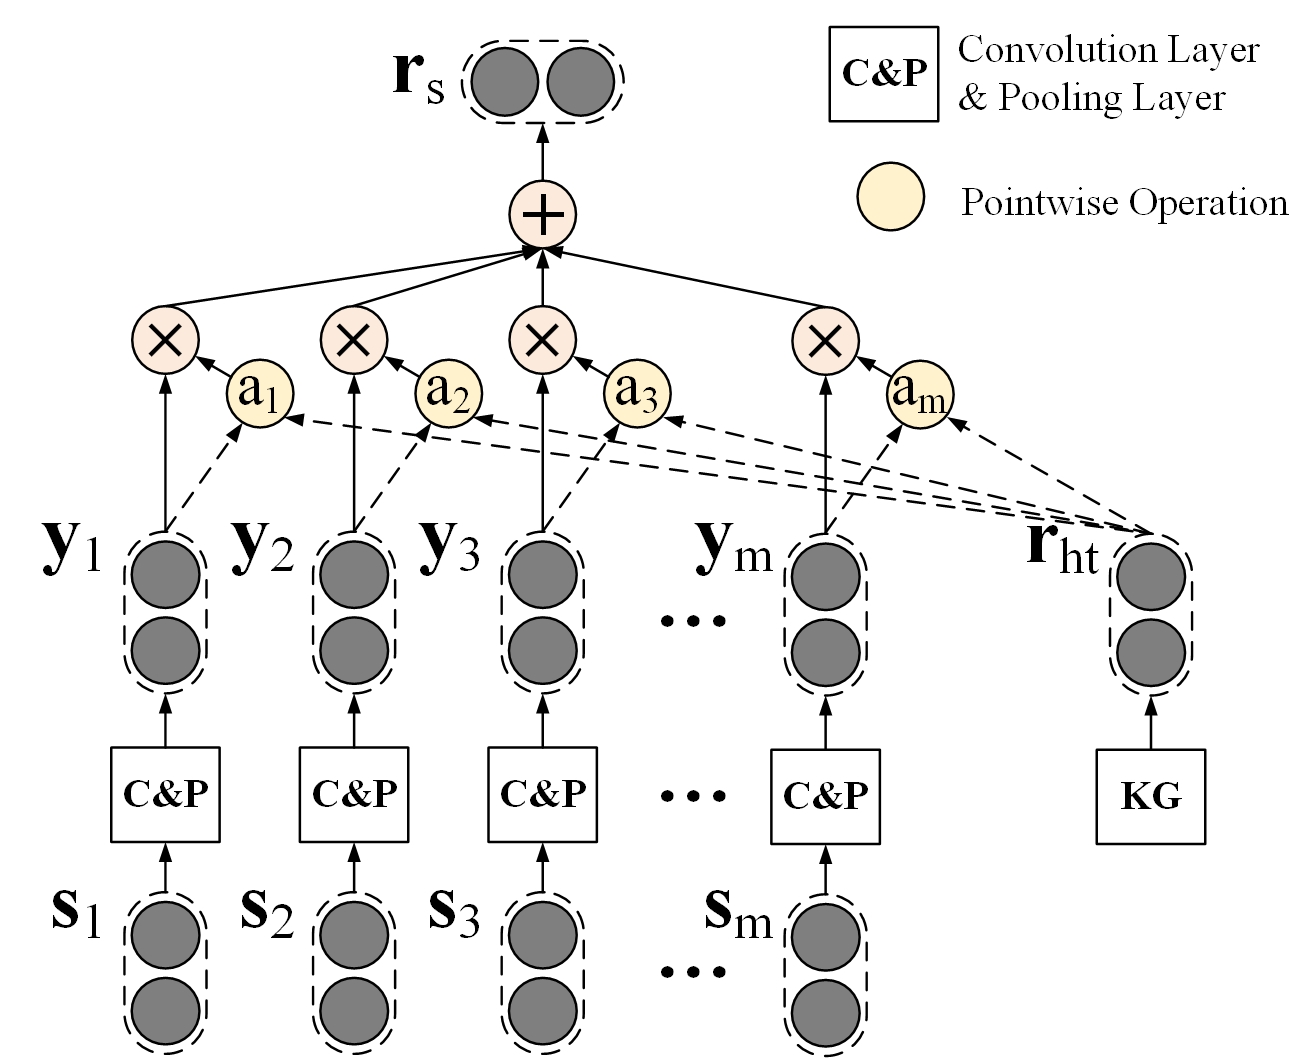
\includegraphics[width=0.9\columnwidth]{figures/ch3/cnn.jpg}
\caption{基于知识注意力机制的卷积神经网络模型}
\label{fig3:cnn}
\end{figure}

图\ref{fig3:cnn}描述了我们卷积神经网络的整个结构,也是文本关系表示学习模型的整个结构。对于任意一个标注了实体对$(h, t)$的句子$s$,如果实体对之间的关系为$r_s$的话,神经网络结构会以句子$s$的词语序列向量$\mathbf{s} = \{\mathbf{x}_1, \ldots, \mathbf{x}_n \}$作为输入。输入的句子向量在通过卷积神经网络中卷积与池化两层操作之后,输出一个文本意义描述的关系向量$\mathbf{y}$。由于存在多个句子标注了相同的实体,我们设置了一个基于知识图谱的注意力机制,用来在这些句子输出向量的基础上进行加权合并,然后得到一个全局的文本关系表示$\mathbf{r}_s$。对于句子的语义信息能在多大程度上描述文本关系,在经过一层多项逻辑斯特回归之后,我们用以下的能量函数来刻画:
\begin{equation}
\mathbf{o} = \mathbf{M}\mathbf{r}_s,
\label{eq3:cnn_distance}
\end{equation}
这里$\mathbf{M} \in \mathbb{R}^{\|R\| \times k_c} $是一个关系表示矩阵用来求得$\mathbf{r}_s$在不同关系上的能量评分,$k_c$是隐层向量的维度,最后我们可以定义一个条件概率$P((s, r_s)|{\theta_V})$:
\begin{equation}
P((s, r_s)|{\theta_V}) = \frac{\exp(\mathbf{o}_{r_s})}{\sum_{r \in R} \exp(\mathbf{o}_{r})}
\label{eq3:cnn_distance1}
\end{equation}

我们的文本关系表示模型就是由这几个部分构成的,包括输入层、卷积层、池化层、基于知识的注意力机制以及刚才介绍的分类层,相关细节将在下面一一展开。有了这些结构之后,我们衡量句子的语义能多大程度上表达某个特定关系就可以迎刃而解了。



\subsubsection{输入层}
 
给定一个含有$n$个单词的句子$s$,$s = \{ w_1, \ldots , w_n\}$,输入层的功能就是将$s$中的所有单词转化成对应的输入词向量$\mathbf{s} = \{ \mathbf{x}_1, \ldots , \mathbf{x}_n \}$。对于给定的句子$s$中任意一个单词$x_i$,其输入向量$\mathbf{x}_i$由两个实向量构成,一个是它的文本词向量$\mathbf{w}_i$,另一个是它的位置向量$\mathbf{p}_{i}$。

文本词向量可以将词的语义信息编码到低维空间中,并且通常会通过大量文本预先训练获得。大量的实验表明,以预先训练好的词向量作为网络输入可以有效提升神经网络的模型效果。在我们的工作中,词向量通过 Skip-Gram \cite{mikolov2013efficient}在大规模文本语料上提前训练获得。

位置向量的概念首次被提出是在 Zeng \cite{zeng2014relation} 的工作中。位置向量是一个可以表明给定单词与句子标注实体之间相隔距离的特征。举个例子,``\emph{马克·吐温}出生于\emph{佛罗里达州}''中,\emph{马克·吐温}与\emph{佛罗里达州}是标注出的实体,\emph{出}离\emph{马克·吐温}和\emph{佛罗里达州}的距离分别为$1$和$-3$。我们会将这些距离也映射到维度$k_p$的连续空间上。对于句子$s$中给定的单词$w_i$,它的位置向量为$\mathbf{p}_i = [\mathbf{p}^h_i, \mathbf{p}^t_i]$, $\mathbf{p}^h_i, \mathbf{p}^t_i \in \mathbb{R}^{k_p}$,其中$\mathbf{p}^h_i$ 和 $\mathbf{p}^t_i$分别是到头实体以及尾实体之间的距离向量。

接着我们合并词向量$\mathbf{w}_i \in \mathbb{R}^{k_w} $与位置向量$\mathbf{p}_i \in \mathbb{R}^{k_p \times 2} $得到最终的输入向量$\mathbf{x}_i \in \mathbb{R}^{k_i} (k_i = k_w + k_p \times 2)$,从而卷积神经网络的输入为:
\begin{align}
\mathbf{s} & = \{\mathbf{x}_1,\ldots, \mathbf{x}_n\} \\\nonumber
&=\{[\mathbf{w}_1;\mathbf{p}_1],\ldots, [\mathbf{w}_n;\mathbf{p}_n]\}.
\end{align}




\subsection{卷积层}

卷积层将输入层得到的句子向量$\mathbf{s}$作为该层的输入,通过卷积层内的操作后导出为隐层向量$\mathbf{h}$。在卷积层中,我们在输入的序列向量$\mathbf{s}$上滑动一个尺寸为$m$的窗口。在每次窗口滑动中,我们可以采样得到一个局部的组合向量$\mathbf{\hat{x}}_i$:
\begin{equation}
\mathbf{\hat{x}}_i = \big[ \mathbf{x}_{i - \frac{m-1}{2}}; \ldots ; \mathbf{x}_i; \ldots ;\mathbf{x}_{i + \frac{m-1}{2}} \big],
\end{equation}
将输入序列$\mathbf{s}$落在以$\mathbf{x}_i$为中心的长度为$m$的窗口中的向量组合,就是这个组合向量$\mathbf{\hat{x}}_i$。如图\ref{fig3:conv_pooling}所示,如果窗口尺寸$m$为$3$,那么连续三个输入向量会组合成一个组合向量。然后,我们将这个组合向量$\mathbf{\hat{x}}_i$进行线性变换以及激活从而得到隐层向量$\mathbf{h}_i$
\begin{equation}
\mathbf{h}_i = \tanh(\mathbf{W}\mathbf{\hat{x}}_i + \mathbf{b}),
\end{equation}
这里,$\mathbf{W} \in \mathbb{R}^{k_c \times mk_i}$是卷积层的卷积核矩阵,$\mathbf{b} \in \mathbb{R}^{k_c}$是卷积层的偏移向量,$k_c$是隐层向量$\mathbf{h}_i$的维度。我们的激活函数选用了$\tanh$,激活的主要作用是将连续信号稳定约束在$[-1,1]$之间。

我们对一句话的理解不是割裂的,而是若干个语义小片段共同建立语义理解的,一个词如果不联系上下文是无法建立准确语义理解的。卷积层的主要物理意义就是在于对语言的局部语义采样,而窗口的大小就是上下文范围的大小。

\vspace{25pt}
\begin{figure}[h]
\setlength{\abovecaptionskip}{30pt} 
\centering
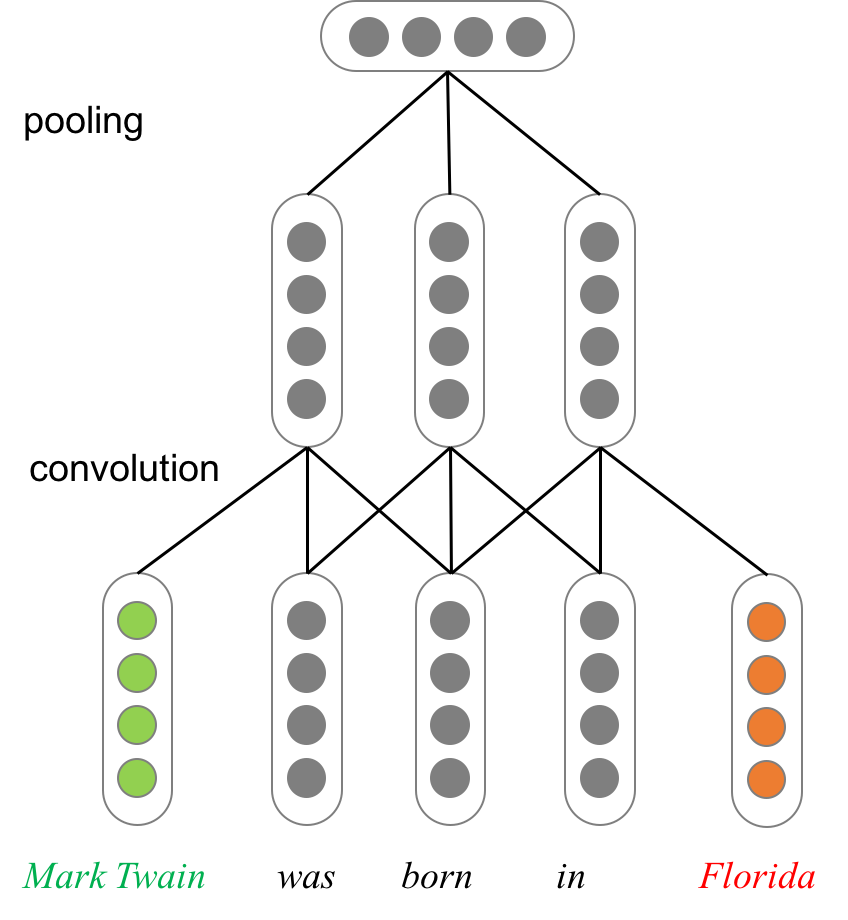
\includegraphics[width=0.7\columnwidth]{figures/ch3/cnn_concrete.png}
\caption{卷积层和池化层的结构示意图}
\label{fig3:conv_pooling}
\end{figure}



\subsection{池化层}

在池化层中,一个最大池化操作在隐层向量${\mathbf{h}_1, \ldots , \mathbf{h}_n}$上被实施,以便获得最后的输出向量$\mathbf{y} \in \mathbb{R}^{k_c} $,具体的过程如下:
\begin{equation}
\mathbf{y}_{j} = \max \{\mathbf{h}_{1,j}, \ldots, \mathbf{h}_{n,j} \},
\end{equation}
这里,$\mathbf{y}_{j}$是输出向量$\mathbf{y}$的第$j$维的值,$\mathbf{h}_{i,j}$是第$i$个隐向量$\mathbf{h}_i$的第$j$维的值。

池化层的主要作用在于对全局的特征进行汇总。在卷积层中,卷积实际上是对局部的语义进行特征提取。但是一个句子的语义仅仅依靠于局部特征是不恰当的,语义的理解最后还是要落实到全局的。池化的作用就是在每个局部采样输出的每个维度上选取一个信号最强值,从而最后能够汇总得到全局的语义特征,这是句子的语义理解中至关重要的一个步骤。如图\ref{fig3:conv_pooling}所示,所有的隐层向量池化输出一个整体的语义向量。

\subsection{基于知识的跨句注意力机制}

对于知识图谱中任意一个三元组$(h, r, t) \in T$,实际上可能存在若干个句子会包含这个三元组中的实体对$(h, t)$,并且这些句子的语义预示着实体对之间具有特定关系$r$。经过输入层、卷积层、池化层的操作后,这些句子已经有了输出向量${\mathbf{y}_1, \ldots , \mathbf{y}_m}$,$m$为包含这些实体对的句子数量。对于这些句子,我们认为其中的某些句子对最后的文本关系表示学习会更具有贡献性,所以我们需要一个机制来选取这些重要的句子同时规避大量句子带来的噪音。

在这里我们通过引入知识图谱中的潜在关系向量$\mathbf{r}_{ht} \in \mathbb{R}^{k_w} $来在神经网络中进行一个基于知识的注意力机制,从而强化重要句子的影响,具体形式如下:
\begin{equation}
\mathbf{e}_j  = \tanh(\mathbf{W}_s\mathbf{y}_j+\mathbf{b}_s)
\end{equation}
\begin{equation}
a_j  =\frac{\exp(\mathbf{r}_{ht}\cdot\mathbf{e}_j)}{\sum_{k = 1}^{m} \exp(\mathbf{r}_{ht}\cdot\mathbf{e}_k)}
\end{equation}
\begin{equation}
\mathbf{r}_s  = \sum_{j = 1}^{m} a_j\mathbf{y}_j
\end{equation}
这里,$\mathbf{W}_s \in \mathbb{R}^{k_w \times k_c}$是一个权重矩阵用来将前几层的输出向量转换到图谱空间中,$\mathbf{b}_s \in \mathbb{R}^{k_w}$则是线性变换的偏移向量。$a_j$是第$j$个句子输出向量$\mathbf{y}_j$在整个注意力机制结算后得到的权重评价。我们通过每个句子输出向量的权重来对这些向量进行加权求和从而得到一个全局的文本关系嵌入表示$\mathbf{r}_s$。有了全局的嵌入向量后,我们可以将向量$\mathbf{r}_s$带入式\ref{eq3:cnn_distance}以及式\ref{eq3:cnn_distance1}中进行分类。

\subsection{初始化及实现细节}
\label{sec3:detail}
在这一部分,我们主要介绍我们的模型在具体训练以及优化过程中的一些细节操作。对于我们以条件概率式\ref{eq3:topeq}为形式的任务目标,我们定义了一个对数似然函数来作为我们的优化目标,
\begin{align}
\mathcal{L}_{\theta}(G, D) & = \log P(G,D|{\theta}) + \lambda \lVert \theta \rVert_2 \\\nonumber
 & = \log P(G|{\theta_E, \theta_R}) + \log P(D|{\theta_V}) \\\nonumber
 & + \lambda \lVert \theta \rVert_2
\end{align}
这里,$\lambda$是一个超参,$\lVert \theta \rVert_2$是一个$L_2$距离的约束条件。我们的所有模型,包括 Prob-TransE 和 Prob-TransD 以及 CNN 都是通过随机梯度下降(stochastic gradient descent,SGD)算法来进行优化。值得注意的是,我们的损失函数的梯度会被传递到输入层的词向量上,因为这样才能将知识图谱的特征嵌入到词向量中。我们设计了一个多线程同步训练的模式来保障图谱和文本两方面的模型同时进行训练。每个线程控制一个模型以及所使用的训练数据。多个模型在内存上共用词、实体以及关系的嵌入表示,且不加锁,梯度则直接反馈到向量上而不考虑竞争问题。

\section{实验设计与结果分析}

我们提出的框架是一个涉及特征融合的联合学习框架,为了体现在框架下进行联合学习之后各个模型的效果提升,我们设计了两个不同任务的实验。第一个是知识图谱补全方向上的链接预测,第二个是文本关系抽取。在试验中,我们将图谱与文本模型联合学习,并将联合学习后的模型分别与各个经典算法进行对比来衡量特征融合的质量。

\subsection{实验设定}

\subsubsection{实验数据集}


\textbf{知识图谱。} 我们选用了 Freebase \cite{bollacker2008freebase} 来作为知识图谱这一块的数据来源。我们在引言中介绍过,Freebase 是一个被广泛利用的大规模知识图谱,并且对公众开放及提供数据下载。在我们的工作中,我们为实验环节引入了两个从 Freebase 中随机抽取的数据集合,包括 FB15K \footnote{https://everest.hds.utc.fr/doku.php?id=en:transe} 和 FB60K。FB15K 已经被很多工作采用并作为一个链接预测的标准测试集合长期存在。FB60K 是一个拓展自 Riedel \cite{riedel2010modeling} 发布的关系抽取文本的图谱数据集合,并且一直被用来进行作为关系抽取的标准数据。我们将 FB15K 和 FB60K 的数据集合详细细节罗列在表\ref{tab3:statistics-of-FB15K}中,包括实体数量、关系数量、事实三元组数量等等。

\vspace{25pt}
\begin{table}[htb]
\setlength{\abovecaptionskip}{30pt} 
\centering
\caption{FB15K 与 FB60K 的数据细节}
\begin{tabular}{|c|c|c|c|}
\hline
数据集合 & 关系 & 实体 & 三元组 \\ \hline
FB15K   & 1345           & 14951            & 592213 \\ \hline
FB60K   & 1324           & 69512            & 335350 \\ \hline
\end{tabular}
\label{tab3:statistics-of-FB15K}
\end{table}

\textbf{文本语料。} 我们从纽约时代周刊杂志(New York Times,NYT)的文章里选择合适的句子作为我们的文本语料。选取句子的方法是 Mintz \cite{mintz2009distant}提出的远距离监督算法(Distant Supervision),只要在一个句子里同时包含有一个三元组的头实体与尾实体,那么这个句子就会被加入我们的文本语料。我们提取了$194385$个同时包含有FB15K中头尾实体的句子,并且将句子标注为头尾实体所对应关系的正例。这些句子覆盖了FB15K中$47103$个事实三元组,共计$699$种关系以及$6053$个实体,我们将这个文本语料命名为 NYT-FB15K,即基于 FB15K 抽取的 NYT 文本语料。而 FB60K 的文本语料则是直接来自于 Riedel \cite{riedel2010modeling}在关系抽取中使用的数据,其中有$570088$个句子,覆盖了$63696$个实体,$56$种关系以及$293175$个事实三元组。我们将这个文本语料命名为 NYT-FB60K。

我们与之前的研究工作保持一致,FB15K 与 NYT-FB15K 用来在链接预测任务中进行评测,FB60K 和 NYT-FB60K 则被用在文本关系抽取这个任务上,这样的设定最大程度的保证了实验的公平性与可操作性。


\subsubsection{图谱文本匹配}
\label{sec3:alignment}

因为文本中的句子不是直接就含有实体标注以及实体关系标注的,所以我们不得不采用一些办法来标注句子中的实体以及实体的文本关系,从而能够支持我们联合学习框架的训练。具体的实施细节我们分为实体文本匹配以及关系文本匹配两个部分。


\textbf{实体文本匹配。}大量知识图谱中的实体出现在文本之中是一个很普遍的现象,而这也是我们试图融合图谱结构特征与文本语义特征的主要出发点。然而,将图谱中的实体与文本中的词相匹配却不是一件容易办到的事情。实体很准确,但是词却不是,一个词可能会指向多个不同的实体。举个例子,一个句子中的\emph{华盛顿},在不考虑上下文的情况下,可以指代美国国父也可以指代美国华盛顿特区。一个是人一个是地点,两者相去甚远。同样,\emph{苹果}可以是科技企业也可以是水果。在这里,我们使用了实体链接技术以及文本之间的锚链接来构建实体与词的匹配。由于文本的数据来源为网络资源,文章间的锚链接往往会指向一个实体,我们使用了这个信息将$E$的实体与词汇表$V$中的词匹配起来 \footnote{在我们的框架中,实体在$\theta_E$中的嵌入与对应词在$\theta_V$的嵌入在空间上是共享的。}。

\textbf{关系文本匹配。}正如我们在前文提到的那样,我们是可以从文本语料之中提取关系特征的。换句话说,关系的嵌入除了从图谱结构学习到之外也可以从文本语料中学习得到。受 Mintz \cite{mintz2009distant} 远距离监督算法的启发,我们也采用类似的方法来进行关系文本匹配。对于给定的一个关系$r \in R$,我们将所有存在关系$r$的实体对聚在一个集合中$Pair_{r} = \{(h, t) | (h, r, t) \in T \}$。然后,如果文本语料$D$中的某个句子同时包含有$Pair_{r}$中某个实体对的头尾实体,那么这句话将会被标注为关系$r$的正例。

\subsubsection{实验与模型参数设置}

在我们的联合框架中,我们从$\{0.1, 0.01, 0.001\}$之中为知识图谱$P(G|{\theta_E,\theta_R})$选择学习率$\alpha_k$,从$\{0.1, 0.01, 0.001\}$之中为文本模型$P(D|{\theta_V})$选择学习率$\alpha_t$。对于卷积神经网络的滑动窗口,我们从$\{3,5,7\}$之中选择滑动窗口的尺寸大小$m$。由于其它的一些参数对于实验影响不是非常大,并且出于实验背景统一与公平的考量,我们直接使用了过去一系列工作\cite{zeng2014relation,lin2016neural}对于卷积神经网络的参数设定。同样是为了与之前的相关工作进行对比,词、实体、关系的嵌入维度$k_w$在关系抽取任务中被设定为$50$,而在图谱填充的链接预测任务中,嵌入维度被设定为$100$。在表\ref{tab3:parameters}中我们罗列了实验中所有的参数细节。

\vspace{25pt}
\begin{table}[h]
\setlength{\abovecaptionskip}{30pt} 
\centering
\caption{联合学习框架参数设置}
\begin{tabular}{|cr|}
\hline
\multicolumn{1}{|c|}{约束系数 $\lambda$}                & 0.0001 \\
\multicolumn{1}{|c|}{知识图谱模型学习率 $\alpha_k$}        & 0.001 \\
\multicolumn{1}{|c|}{文本模型学习率 $\alpha_t$}             & 0.01  \\
\multicolumn{1}{|c|}{隐层向量维度 $k_c$}        & 230   \\
\multicolumn{1}{|c|}{词、实体、关系嵌入维度 $k_w$} & 50    \\
\multicolumn{1}{|c|}{位置向量维度 $k_p$}            & 5     \\
\multicolumn{1}{|c|}{窗口尺寸 $m$}    & 3     \\
\multicolumn{1}{|c|}{梯度传播中断概率 $p$}            & 0.5  \\
\hline
\end{tabular}
\label{tab3:parameters}
\end{table}



\subsection{关系抽取实验结果}

\subsubsection{测试结果}

在大量的工作中 \cite{mintz2009distant,riedel2010modeling,hoffmann2011knowledge,surdeanu2012multi,zeng2014relation,zeng2015distant,lin2016neural},文本模型都是用已有的知识图谱进行远距离监督,来自动地从文本中标注句子并加入到训练样例集合之中。从这些自动构建的训练数据中模型可以抽取语义特征并构建一个关系的分类器。我们也在这个机制上进行实验,以便评估联合学习对文本模型的效果提升。

我们采用了 Weston \cite{weston2013connecting}的实验设定来进行测试。严格意义上讲,关系抽取不是一个单分类任务,而是一个多分类任务。在测试过程中,对于测试实体对,我们会将所有的关系都作为候选与实体对进行计算。模型会给出每种关系在语义信息下与测试实体对的对应程度,并获得评分。一个关系,如果与实体对构成的三元组在知识图谱内,则为正确预测,反之为错误预测。测试系统会将评分进行排序,并且根据召回率与准确率的曲线来评估模型效果。

在 NYT-FB60K 数据集上的测试结果都被罗列在图\ref{fig3:jointcnn}中。图中``JointD+KATT''表示与 Prob-TransD 联合学习后具有知识导向注意力机制的卷积神经网络模型;``JointE+KATT''表示与 Prob-TransE 联合学习后具有知识导向注意力机制的卷积神经网络模型;``CNN+ONE''表示使用了 at-least-one 机制 \cite{zeng2015distant} 的卷积神经网络模型;``CNN+ATT''表示使用了句子级别注意力机制 \cite{lin2016neural} 的卷积神经网络模型,也是当前在关系抽取任务上效果最好的模型。除此以外,我们也将这一系列神经网络模型与经典的基于统计的关系抽取文本模型进行了对比,这些模型包括 Mintz \cite{mintz2009distant}、MultiR \cite{hoffmann2011knowledge}、MIML \cite{surdeanu2012multi} 以及 Sm2r \cite{weston2013connecting}。结果同样被罗列在图\ref{fig3:jointcnn}中。

\begin{figure}[h]
\centering
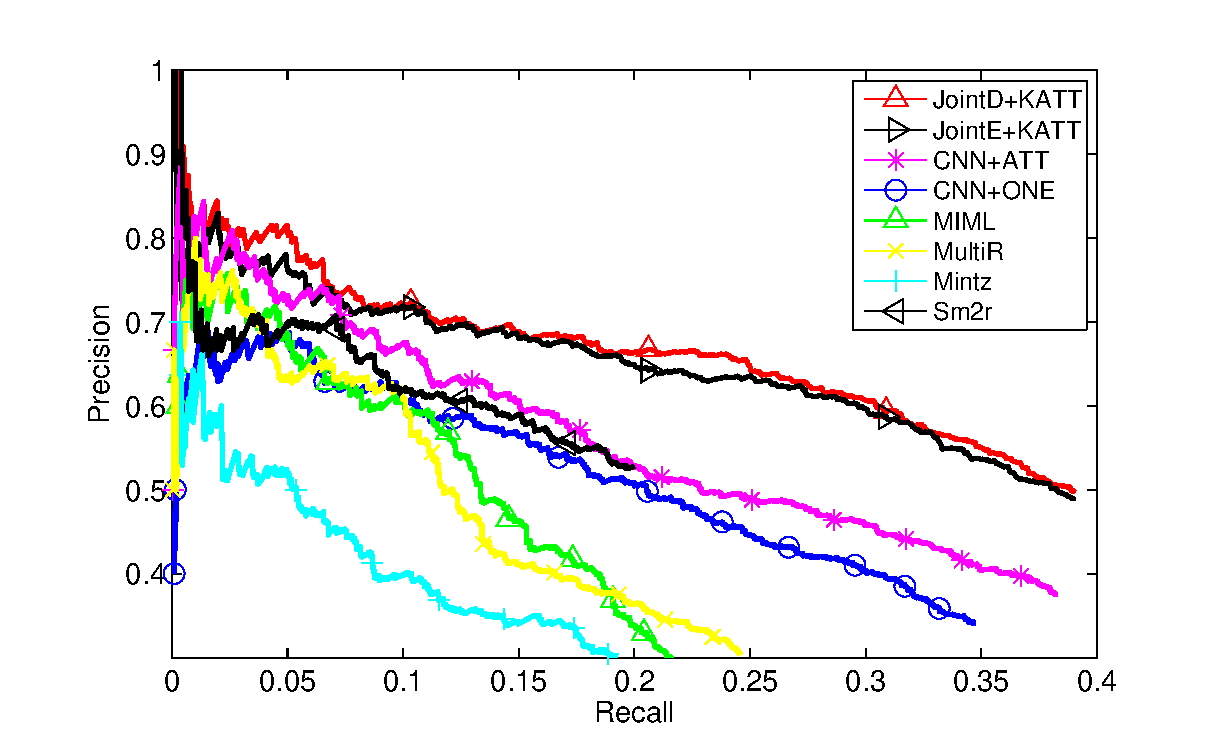
\includegraphics[width=0.9\columnwidth]{figures/ch3/res.eps}
\caption{JointD+KATT、JointE+KATT、CNN+ATT、CNN+ONE、MIML、MultiR、Mintz 与 Sm2r 的准确率/召回率曲线}
\label{fig3:jointcnn}
\end{figure} 

从实验结果中我们可以得出以下几个结论:

(1)与图\ref{fig3:jointcnn}中各个模型相比,经过联合学习框架训练之后的文本模型在整个召回率区间上都取得了最高的准确率,并且在效果上显著高出其余所有模型。当召回率大于$0.15$时,联合学习框架训练后的模型整体提升准确率在$10\%$到$20\%$之间。当召回率小于$0.15$时,模型也取得了最好的效果,并且比其余模型更为稳定。总的来说,联合学习模式下特征融合带来的受益在文本模型上体现的十分明显。

(2)除了 JointD+KATT、JointE+KATT 之外,CNN+ATT、CNN+ONE 与基于统计的模型相比,在召回率超过$0.15$的时候同样取得了超过$10\%$的准确率提升。并且整体上来看,神经网络模型准确率下降的速度要慢的多。这些实验结果很好的证明了深度神经网络没有局限在特征工程上,并且能够自行从原始数据中挖掘特征,稳定又有效。

(3)尽管基于统计的模型准确率都下降的非常快,尤其是与一系列神经网络模型相对比。但是在最高置信度的推荐中,即从$0$开始的一段召回率上,这些模型同样能够得到非常不错的准确率。这说明了,虽然人为设计的特征在某些方面存在局限性,但还是十分有效的。统计模型的主要优势在于其计算规模往往很小,且不需要过多的训练数据,但是有效特征需要人为构建与挑选。这些统计模型训练难度比基于神经网络的模型要简单的多,将两者进行结合并用于我们的工作,将是未来我们继续改进的一个重要方向。

\vspace{25pt}
\begin{table*}[h]
\setlength{\abovecaptionskip}{30pt} 
\centering
\caption{不同模型组合情况下的 P@N 评估结果(\%).}
\begin{tabular}{|c|ccc|ccc|} 
\hline
P@N(\%) & \multicolumn{3}{c|}{100}                                      & \multicolumn{3}{c|}{300} \\ \hline
& \multicolumn{1}{c|}{ONE} & \multicolumn{1}{c|}{ATT} & KATT & \multicolumn{1}{c|}{ONE} & \multicolumn{1}{c|}{ATT} & KATT \\ \hline
CNN+	& 67.3	& \textbf{76.2}	& -     & 58.1	& 59.8 	& -    \\ \cline{1-1}
JointE+  & 67.5 	& 74.1	& 75.8  & 63.0 	& 63.2 	& 68.0  \\ \cline{1-1}  
JointD+  & \textbf{68.5}    & 74.6  & \textbf{80.6}  & \textbf{67.0} & \textbf{67.3} & \textbf{68.7}  \\ \hline
P@N(\%) & \multicolumn{3}{c|}{500}                                      & \multicolumn{3}{c|}{Mean} \\ \hline 
& \multicolumn{1}{c|}{ONE} & \multicolumn{1}{c|}{ATT} & KATT & \multicolumn{1}{c|}{ONE} & \multicolumn{1}{c|}{ATT} & KATT \\ \hline
CNN+	& 43.7	& 48.5			& -     & 56.4 	& 61.5 	& -     \\ \cline{1-1}
JointE+  & 57.3 	& 59.3 	& 63.0  & 62.6 	& 65.5  & 68.9  \\ \cline{1-1}
JointD+  & \textbf{58.6}    & \textbf{61.1}  & \textbf{63.7}  & \textbf{64.8}   & \textbf{67.7}    & \textbf{71.0}  \\ \hline
\end{tabular}
\label{tab3:relationExt}
\end{table*}


\subsubsection{联合学习及基于知识的注意力机制的定量分析}

编码器至少一个机制(ONE),句子级注意(ATT)和我们基于知识的关注(KATT)。 “JointD”和“JointE”分别表示与Prob-TransD和Prob-TransE共同学习的CNN模型,“CNN”表示没有联合学习的CNN模型。 结果显示在表\ ref {tab3:relationExt}中,包括P @ 100,P @ 200,P @ 300及其平均值。

对于关系抽取,我们通常会更加注意那些具有最高置信度得分的推荐。毕竟我们并不指望模型能够达到十全十美,高置信度的推荐保持一个很好准确率其实更符合我们的应用需求。为了能够更详细地比较联合学习前后模型结果上的变化,我们采用了另一种评估推荐效果的测试方式。我们将推荐得分排序后,选取最高置信度的若干个推荐,此时预测的准确率将作为我们衡量模型能力的指标。

在这个实验中,我们选择 Zeng \cite{zeng2014relation} 使用过的卷积神经网络作为文本编码的模型。卷积神经网络编码器将会与不同种类的跨句学习机制相结合,包括 at-least-one 机制(ONE),句子级别注意力机制(ATT)以及我们的基于知识的注意力机制(KATT)。这样的组合可以对各个跨句合并机制进行定量分析。

我们也将文本模型与知识图谱表示学习模型相结合,从而定量分析联合学习带来的影响。``JointD''表示与 Prob-TransD 联合学习之后卷积神经网络得到的文本模型,``JointE''表示与 Prob-TransE 联合学习之后卷积神经网络得到的文本模型,``CNN''表示没有与知识图谱进行联合学习的卷积神经网络文本模型。具体各种组合的效果被罗列在表\ref{tab3:relationExt}中,包括前$100$推荐准确率P@100、 前$300$推荐准确率P@300、前$500$推荐准确率P@500以及准确率的平均值。

从实验结果我们可以得出以下几点:

(1)所有的文本编码器,无论是采用哪种跨句学习机制,在联合学习框架下进行训练之后,都在效果上有大幅度的提升。从平均的推荐准确率来看,联合学习后 CNN+ONE 的准确率提升了$6\%$左右,而 CNN+ATT 的准确率也提升了$5\%$左右。实验结果表明,我们提出的平行联合学习框架在效率提升之外,特征融合也得到了保障,联合学习后文本模型接收到图谱的影响提升了自身的推荐效果。


(2)比起与Prob-TransE进行联合学习的文本编码器,与Prob-TransD进行联合学习的文本编码器进一步提升了推荐效果。Prob-TransD是一个比Prob-TransE更复杂,更具有表达能力的知识图谱表示学习模型,并且可以更好地提取知识图谱特征以及理解实体之间关系的多样性。毕竟,在Prob-TransD中,实体在不同关系的环境下是具有不同的嵌入的,这可以更好地满足图谱中多样性的表达需求。实验结果也表明,联合学习框架可以利用图谱辅助训练文本模型,并且对图谱模型的适应性很好。图谱模型的效果也影响特征融合的效果,表达能力越强的图谱模型对文本模型的效果提升越明显。

(3)在表\ref{tab3:relationExt}中,注意力式的跨句合并机制 ATT、KATT 比单纯的 ONE 机制要有效的多。训练过程中所使用的文本语料是基于远距离监督机制自动抓取构建的,在构建过程中会引入大量杂质和噪音。这很好理解,一个实体对如果出现在一个句子中,这个句子很有可能在语义上无法描述实体间的关系。而注意力机制能够获取到最有意义的句子并从这个句子里学到更有意义的嵌入,所以在效果上比简单的特征合并要高出许多。


(4)ATT 和 KATT 的比较进一步表明,在跨句合并机制上,不使用知识图谱信息的简单注意力机制还是略显薄弱的。即使是含有相同关系的不同实体对,实体间的关系都有着细微的差别,这与我们在前文提到的实体多样性以及关系多样性有关。ATT 中通过一个模糊的全局向量来进行重要的句子选择,显然这是无法满足关系多样性的特性的。在这里,我们将知识图谱的信息融入到注意力机制中。对于不同的实体对,我们给出局部的向量来进行重点句子选择,而这些局部向量在全局上又密切相关。因此,我们基于知识的注意力机制比直接跨句的简单注意力机制更具有区分度与甄别能力。

\subsection{图谱填充实验结果}

针对实体的链接预测被广泛地使用在知识图谱填充任务中\cite{bordes2013translating,wang2014transh,lin2015learning}。在这里,我们的任务设置和章节\ref{cha2:framework}中链接预测是一致的,给定一个头实体和关系的组合$(h, r, ?)$来预测对应的尾实体,或者给定一个尾实体和关系的组合$(?, r ,t)$。

对于每个测试的三元组$(h,r,t)$,我们用FB15K中的所有实体来替换头实体或者尾实体,按照公式\ref{eq3:kg_distance}计算出评分后以降序排列。依照我们对模型的设想,事实三元组$(h,r,t)$如果成立的话,其对应的评分应当比替换后所有的三元组都要高。我们遵循以往工作一贯的设定,使用正确实体能量得分排在前十的比例来衡量预测质量,我们将这个结果称为$10$预测命中率(Hits@10)。

Bordes\cite{bordes2013translating} 在其工作中将知识图谱中的关系划分为四个大类:一对一(1-to-1)、一对多(1-to-N),多对一(N-to-1)、多对多(N-to-N)。实验也在这四类关系上分别进行了测试与分析。我们同样汇报了不同关系类别上的 Hits@10 结果,包括头实体预测、尾实体预测两个任务方向。除此以外,我们汇报了三元组级别的平均准确率用以刻画模型整体的效果。

由于实验的设定是相同的,所以我们直接从相关工作\cite{bordes2011learning,bordes2012joint,bordes2013translating,wang2014transh,lin2015learning,ji2015knowledge}中引用了 SE、SME、TransE、TransH、TransR、CTransR、TransD 在 FB15K上的实验结果。我们自己动手实现了 TransD,并使用 Github 上 KB2E\footnote{https://github.com/thunlp/KB2E}工具包来实现其他的一些图谱模型。在我们的框架中,没有进行联合学习的知识表示模型被称为``Prob-TransE''和``Prob-TransD'',与卷积神经网络文本模型一起进行联合学习的知识表示模型被命名为``JointE''和``JointD''。具体实验结果显示在表\ref{tab3:entity}之中。

为了进一步论证我们联合框架的有效性,我们也通过关系级别的平均 Hits@10 准确率来刻画模型整体的效果。在关系级别的平均准确率上,Prob-TransE 与 JointE 的结果分别为$\textbf{66.2\%}$和$\textbf{80.4\%}$。Prob-TransD 和 JointD 的结果分别为$\textbf{71.4\%}$和$\textbf{85.1\%}$。


\vspace{25pt}
\begin{table*}[h]
\setlength{\abovecaptionskip}{30pt} 
\centering
\caption{头尾实体链接预测的结果(\%).}
\scalebox{0.90}{
\begin{tabular}{|c|cccc|cccc|c|}
\hline
度量方法            & \multicolumn{4}{c|}{Predicting Head} & \multicolumn{4}{c|}{Predicting Tail} & \multicolumn{1}{c|}{Overall} \\ \hline
类别  & 1-to-1     & 1-to-N    & N-to-1    & N-to-N    & 1-to-1     & 1-to-N    & N-to-1    & N-to-N  & Triple Avg. \\ \hline

SE \cite{bordes2011learning}&35.6 &62.6 &17.2 &37.5 &34.9 &14.6 &68.3 &41.3 &39.8  \\ 
SME \cite{bordes2012joint}&35.1 &69.6 &19.9 &40.3 &32.7 &14.9 &76.0 &43.3 &41.3  \\ 
TransE \cite{bordes2013translating}            & 43.7       & 65.7      & 18.2      & 47.2      & 43.7       & 19.7      & 66.7      & 50.0    & 47.1  \\ 
TransH \cite{wang2014transh}    & 66.8       & 87.6      & 30.2      & 64.5      & 65.5       & 39.8      &83.3      & 67.2    & 64.4  \\ 
TransR \cite{lin2015learning}   & 78.8       & 89.2      & 38.1      & 66.9      & 79.2       & 38.4      &90.4      & 72.1    & 68.7  \\ 
CTransR \cite{lin2015learning}    & 81.5      & 89.0      & 36.4      & 71.2      & 80.8       & 38.6      &90.1      & 73.8    & 70.2  \\ 

TransD \cite{ji2015knowledge} &81.2  &94.8  &47.1 &79.3  &81.6 &53.9 &93.7 &82.5  &78.9  \\ \hline


Prob-TransE      & 66.5       & 88.8      & 39.8      & 79.0      & 66.4       & 51.9      & 85.6      & 81.5    & 76.6  \\
JointE     &82.7 & \textbf{96.2} &45.0 &80.7 &81.7& 57.7 & 93.6 &84.0 & 79.3  \\ \hline

Prob-TransD		&79.1	&93.0 &42.2	&79.2	&79.2	&51.6	&90.9	&82.7	&78.2  \\  

JointD    &\textbf{82.7}   &95.2 &\textbf{47.8} & \textbf{81.6} &\textbf{82.0} &\textbf{57.9} & \textbf{94.7} &\textbf{84.7} & \textbf{80.4}  \\ \hline
\end{tabular}}
\label{tab3:entity}
\end{table*}


从实验结果我们可以观察到以下几点:

(1)无论是预测头实体,还是尾实体,联合学习框架下的图谱模型在四大类关系上几乎都得到了的改善。特别是,Joint-TransE 与 Joint-TransD 比起 Prob-TransE 和 Prob-TransD,在关系级别的平均准确率上实现了超过$10\%$的提升。这表明,联合学习之后对知识图谱嵌入表示带来的提升是一致且鲁棒的,并且在框架下与文本模型一起学习的知识图谱表示模型可以很好的利用文本语义与文本关系的对应来提升关系层次的表达能力。

(2)与多对多的关系相比,一对一、一对多以及多对一关系上,联合学习框架下学习得到的模型提升效果更为明显。这表明我们联合学习框架融入的文本特征,对确定性关系的嵌入有很好的帮助。在数据集合 FB15K 中,超过$80\%$的三元组属于多对多关系的实例。由于联合学习模型在多对多关系上的效果提升没有其他类别关系上显著,因此在三元组级别的平均准确率上,提升没有关系级别的平均准确率突出。

(3)TransD 是 TransE 的扩展的模型,具有更复杂的实体嵌入机制。在 TransD 中,每个实体在不同的关系空间中具有不同的嵌入表示。与其他的模型相比,TransD 可以取得更好的实验结果。而在联合学习框架中与文本模型一起学习后,TransD 进一步提高了效果。这些结果意味着与 TransE 和 TransD 相似的其他知识图谱表示学习模型,如 TransH、TransR 等,都可以用类似的方法与我们的框架进行整合。

\section{本章小结}

在本章节中,我们提出了一个通用的联合学习框架来将知识图谱与文本模型进行结合。我们的联合学习框架将实体、关系和文本词汇嵌入到统一的连续空间中,并通过这样的方式来进行特征融合。更进一步,我们采用了图谱文本匹配以及基于知识的注意力机制来交换知识图谱模型与文本模型之间的信息。值得注意的是,以往的模型多是串行结合的模式,而我们采用了并行结合的模式以便在训练效率上有大幅度提升。在实验阶段,我们使用关系抽取来度量文本模型,使用链接预测来度量图谱模型。实验结果表明,我们平行的联合学习框架可以有效学习知识图谱与文本的嵌入表示,并且得到的嵌入更具有区分性与辨识度。通过结合不同的知识图谱表示学习模型,我们证明了联合框架对现有图谱模型的开放性,不同的图谱模型都可以被吸收进入框架。在未来的工作中,我们将尝试使用高效的实现方式来将循环神经网络 RNN 用作文本编码器。与统计模型相结合以及融入更多的特征作为联合框架的指导,比如图谱的关系路径、文本的语法关联,也是非常有意义的尝试方向。







